\section{Ergonomia de carregamento de peso}

Considerando a configuração do projeto, é possível que seja necessário o levantamento e carregamento da transportadora em algumas situações durante o transporte. Portanto, deve-se levar em conta as regras de ergonomia relacionadas a essa atividade para assegurar a segurança do trabalho. Esse fator vai definir principalmente o peso total limite do projeto.

A CLT (Consolidação das Leis do Trabalho), art. 198/199, e Convenção OIT n.127, determinam um limite de 60 kg para homens e 25 kg para mulheres. Entretanto, a forma como esse padrão foi definido não leva em conta fatores importantes como a diferença do tipo de carga. E a NR 17, Norma Regulamentadora que trata de ergonomia, não define um peso de carregamento. Portanto, não existe um peso de limite de carregamento muito bem definido. \cite{ergotriade2016}

Um método frequentemente utilizado para definir esse peso é a Equação NIOSH, concebida pelo National Institute for Occupational Safety and Health, nos Estados Unidos. Esse método define um peso limite para carregamento de cargas de 23 kg em condições ideais, que pode ser diminuído de acordo com as condições de carregamento e trabalho.

\begin{equation}
LPR = LC \times HM \times VM \times DM \times AM \times FM \times CM
\end{equation}

em que LPR é o limite de peso recomendado e, para os parâmetros do projeto:

\begin{itemize}
\item LC (Constante de Carga) = 23 kg
\item HM (Fator de Distância Horizontal) = 1
\item VM (Fator de Altura) = 0,9
\item DM (Fator de Deslocamento Vertical) = 1
\item AM (Fator de Assimetria) = 0,9
\item FM (Fator de Freqüência) = 1
\item CM (Fator de Pega) = 1
\end{itemize}

Portanto, o limite de peso recomendado por pessoa é de 18,65 kg. Espera-se que a transportadora seja carregada por duas pessoas. Portanto o limite de peso sugerido para o projeto é de 37,3 kg.


\section{TERMOVIDA – Caixa térmica para transporte de órgãos para transplantes}

O projeto TERMOVIDA consiste em uma caixa térmica para transporte de órgãos para transplantes com um sistema de refrigeração autônoma.

A legislação da ANVISA regulamenta como deve se dar o transporte de órgãos para transplante, as informações que devem ser coletadas que constatam o tempo de vida e a temperatura ideal a ser mantida para que os órgãos que sejam transportados em segurança por este dispositivo puderam indicar como deve ser o recipiente e quais sao os equipamentos necessário para que o mesmo funcione corretamente.

Neste projeto, é utilizada uma pastilha de efeito Peltier para a refrigeração da caixa, controlada por histerese, via um micro-controlador. O equipamento, utilizado durante o transporte em veículos, utiliza alimentação elétrica do sistema de 12V do veículo.

A estrutura da caixa é feita de material isolante térmico. Esta possui uma porta de ventilação na lateral, onde está posicionada a pastilha Peltier, e um espaço no qual um painel LCD sensível ao toque está alocado. O painel é responsável por mostrar as condições monitoradas.

\begin{figure}[H]
\centering
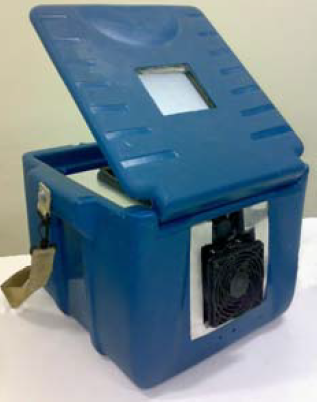
\includegraphics[scale=1]{figuras/termovida.png}
\caption{TERMOVIDA - Caixa térmica para transporte de órgãos para transplantes}
\end{figure}